\chapter{Терминология}

\section{Интеллектуальный агент}

\begin{figure}[h]
\centering
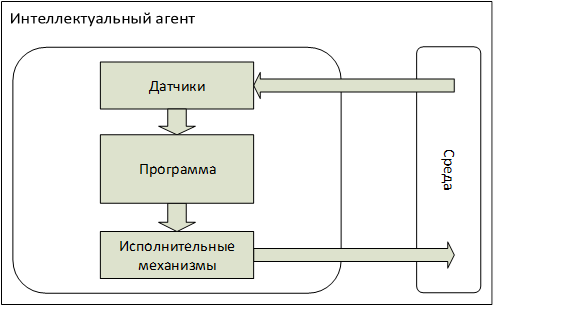
\includegraphics{agent.png}
\caption{Общая схема устройства интеллектуального агента}
\end{figure}



\emph{Агентом} будем называть сущность, которая воспринимает окружащую
ее среду с помощью датчиков и воздействует на нее исполнительными
механизмами.

Термином \emph{восприятие} обозначаются полученные агентом сенсорные
данные в любой конкретный момент времени.

\emph{Последовательностью актов восприятия} агента называется полная
история всего, что было когда-либо им воспринято.

\section{Проблемная среда}

Для полного описания агента и среды, в которой он действует,
предлагается использовать классическую формулировку проблемных сред по
схеме PEAS:

\begin{itemize*}
\item
  Performance -- \emph{критерии производительности}, которые стремиться
  максимизировать агент
\item
  Environment -- \emph{описание окружающей среды}, предметной области
\item
  Actuators -- \emph{исполнительные механизмы}, или действия
\item
  Sensors -- доступные агенту \emph{датчики}
\end{itemize*}

\subsection{Рациональный агент}

Сформулируем важное определение, опираясь на введенные критерии: для каждой возможной последовательности актов восприятия
\emph{рациональный агент} должен выбрать действие, которое, как
ожидается, максимизирует его показатели производительности, с учетом
фактов, предоставленных данной последовательностью актов восприятия и
всех встроенных знаний, которыми обладает агент.

\subsection{Классификация}

Проблемные среды классифицируются по ряду признаков:

\begin{description}
\item[Полностью или частично наблюдаемая] \hfill \\
  Среда называется полностью
  наблюдаемой, если датчики агента предоставляют ему доступ к полной
  информации о состоянии среды в каждый момент времени. Частичная
  наблюдаемость может возникнуть, например, из-за создающих шум или
  неточных датчиков или из-за того, что отдельные характеристики ее
  состояния отсутствуют в информации, получаемой от датчиков.
\item[Детерминированная или стохастическая] \hfill \\Если следующее состояние среды
  полностью определяется текущим состоянием и действием, выполненным
  агентом, то такая среда называется детерминированной. В противном
  случае она является стохастической. Может создаться впечатление, что
  среда стохастическая в случае, когда она является частично
  наблюдаемой.
\item[Эпизодическая или последовательная] \hfill \\В эпизодической среде опыт агента
  состоит из неразрывных эпизодов. Каждый эпизод включает в себя
  восприятие среды агентом, а затем выполнение одного действия. При этом
  каждый следующий эпизод не зависит от действий,\\предпринятых в
  предыдущих. В противоположность этому, в последовательных вариантах
  среды каждое текущее решение может повлиять на все будущие.
\item[Статическая или динамическая] \hfill \\Если среда может измениться в ходе того,
  как агент выбирает очередное действие, то такая среда называется
  динамической для данного агента, в противном случае -- статической.
\item[Дискретная или непрерывная] \hfill \\Различия между дискретными и непрерывными
  средами относятся к описанию состояния, способу учета времени,
  восприятиям и действиям агента.
\item[Одноагентная или мультиагентная] \hfill \\Иногда целесообразно рассматривать
  пользователя как второго агента.
\end{description}

\section{Пропозициональная логика}

При обсуждении условного планирования используется язык \emph{пропозицио\-нальной логики} (лат. propositio --- «высказывание»). Это раздел символической логики,
изучающий сложные высказывания, образованные из простых, и их
взаимоотношения. С точки зрения выразительности, логику высказываний
можно охарактеризовать как классическую логику нулевого порядка.

\subsection{Язык}

Алфавит языка разделен на три группы.

\begin{itemize*}
\item
  Пропозициональные переменные: $A, B, C, ...; A \in \{0, 1\}$;
\item
  Логические союзы: : $\neg$ --- знак отрицания, $\land$ --- знак
  конъюнкции, $\lor$ --- знак дизъюнкции, $\implies$ --- знак
  импликации, $\iff$ --- знак эквивалентности;
\item
  технические знаки: ( --- левая скобка, ) --- правая скобка.
\end{itemize*}

Сам язык можно индуктивно определить следующим образом:
\begin{enumerate}
 \item пропозициональная переменная есть формула;
 \item если $A$ -- произвольная формула, то $\neg A$ -- тоже формула;
 \item если $A$ и $B$ -- произвольные формулы, то $(A \implies B)$, $(A \land B)$, $(A \iff B)$, $(A \lor B)$ -- также формулы
\end{enumerate}

\subsection{Выполнимость булевых формул}

При работе с высказываниями пропозициональной логики возникает
\emph{задача выполнимости булевых формул}, SAT\footnote{Boolean Satisfability problem}, которая формулируется так:
можно ли назначить всем переменным, встречающимся в формуле, значения
ложь и истина так, чтобы формула стала истинной. Известно, что эта
задача в общем случае обладает свойством $NP$-полноты.

\section{Условное планирование}

Далее приводятся сведения о планирующих агентах, действующих в частично
наблюдаемой, динамической, одноагентной среде.

\subsection{Язык PDDL}

Стандартом де-факто для описания задач планирования является язык
PDDL\footnote{Planning Domain Definition Language}. Основными его понятиями являются проблемная среда и
задача (проблема), поставленная на ней в виде начального и конечного
состояний. В дальнейшем понятия проблемная среда и предметная область будут рассматриваться как взаимозаменяемые.

В описании проблемной среды положим, что ее состояние задано набором
признаков. Для простоты будем все признаки полагать бинарными. Каждый
возможный набор их значений называется физическим состоянием среды.
Далее, представим датчики агента как акты восприятия значений одного или
более признаков. Исполнительные механизмы будут представлять собой
действия, переводящие среду из одного физического состояния в другое.

Проблемной среде исоответствуют следующая конструкция языка:

\begin{verbatim}
(define (domain <name>)
    <description>
)
\end{verbatim}

\subsection{Пример: мир Лампы}

Для более наглядного обсуждения планирующих агентов введем ``игрушечную'' проблему, которую неформально можно описать следующим образом: в некой
комнате находится лампа накаливания, соединенная выключателем с
источником питания. Там же находятся кондиционер и окно (считаем, что на
улице ночь). Необходимо включить свет.

\subsection{Доверительное состояние}

Более формально, введем набор бинарных признаков, описывающих среду:

\begin{itemize}
\item
  $L$. Свет горит (не горит)
\item
  $B$. Лампа исправна (неисправна)
\item
  $S$. Выключатель включен (выключен)
\item
  $W$. Окно открыто (закрыто)
\item
  $C$. Кондиционер включен (выключен)
\end{itemize}

Тогда например, состояние среды в котором лампа исправна, выключатель
выключен и свет не горит, представляет собой четыре различных физических
состояния:

\begin{equation}\langle \neg L, B, \neg S, \neg W, \neg C\rangle, \langle \neg L, B, \neg S, \neg W, C\rangle, \langle \neg L, B, \neg S, W, \neg C\rangle, \langle \neg L, B, \neg S, W, C\rangle,\end{equation}

Они получены перебором различных значений последних двух признаков.
Введем понятие доверительного состояния среды как подмножества множества
ее физических состояний. Для записи признаков, чье значение неизвестно,
введем сокращенную запись

\begin{equation}A?=A \lor \neg A\end{equation}

Тогда запись выше можно сократить до:

\begin{equation}\langle \neg L, B, \neg S, W?, C?\rangle\end{equation}

В PDDL для описания признаков используется следующая конструкция:

\begin{verbatim}
(: predicates (L) (S) (B) (W) (C) )
\end{verbatim}

Формализуем также описание задачи, задав начальное и конечное состояние
в виде логических формул:

\begin{verbatim}
(define (problem <name>)
    (: domain <domain_name> )
    (: init (~L) )
    (: goal (L) )
)
\end{verbatim}

\subsection{Действия}

Далее, введем действия, позволяющие изменять значения признаков.
Понятно, что в реальной среде не каждое действие доступно для выполнения
в любой момент времени. Поэтому вводятся понятия \emph{предусловия} и
\emph{эффекта} действия как логических выражений с переменными в
множестве признаков. Если текущее физическое состояние не совпадает с
предусловием действия, то его применение не принесет никакого эффекта.

\begin{table}[h]
\begin{tabular}{l | l | l | p{5cm} }
\hline
Действие & Описание & Предусловие & Эффект \\
\hline
$chbulb$ & Заменить лампу & Выключатель выключен & Лампа исправна \\
$brbulb$ & Разбить лампу & Лампа исправна & Лампа неисправна. Свет не
горит \\
$onlight$ & Включить выключатель & Нет & Выключатель включен. Если лампа
исправна, свет горит \\
$offlight$ & Выключить выключатель & Выключатель включен & Выключатель
выключен. Свет не горит \\
$onwind$ & Открыть окно & Окно закрыто & Окно открыто \\
$offwind$ & Закрыть окно & Окно открыто & Окно закрыто \\
$oncond$ & Включить кондиционер & Кондиционер выключен & Кондиционер
включен \\
$offcond$ & Выключить кондиционер & Кондиционер включен & Кондиционер
выключен \\
\hline
\end{tabular}
\caption{Описание действий доступных в мире Лампы}
\end{table}

В PDDL действия содержатся в описании предметной области и задаются
следующей конструкцией:

\begin{verbatim}
    (: action ch_bulb ;Заменить лампу
        :precondition (B? & ~S)
        :effect (B)
    )
\end{verbatim}

Для заданного доверительного состояния выполнимость предусловия
какого-либо действия может быть неизвестной. Например, в состоянии
$\langle\neg L, B?, S?\rangle$ результатом действия $chbulb$ может оказаться как то же самое состояние
в случае, когда $S$ положителен, так и состояние
$\langle\neg L, B, \neg S\rangle$, когда предикат отрицателен.

\subsection{Аксиомы}

Можно заметить, что описания действий содержат дублирующуюся информацию.
Язык PDDL содержит понятие аксиомы - логической формулы, справедливой в
любом доверительном состоянии. Для мира Лампы справедлива следующая
аксиома: свет горит тогда и только тогда, когда лампа исправна и
выключатель включен.

\begin{equation} L \iff B \land S \end{equation}

Ей соответствует конструкция языка:

\begin{verbatim}
(: axiom (L <-> B & S) )
\end{verbatim}

\nameref{sec:appendix_problems} содержит полный вариант PDDL-описания мира Лампы.

\subsection{План -- граф доверительных состояний}

Так как мы рассматриваем частично наблюдаемые среды, то будем считать,
что агенту недоступно восприятие значений каких-либо признаков напрямую.
Результатом работы планировщика будет граф, отображающий возможные пути
из начального доверительного состояния в целевое. Классическим способом
представления неопределенности результата действия, рассмотренного
ранее, является $AND$-$OR$ граф.

\begin{algorithm}
  \caption{Алгоритм построения AND-OR графа}
  \begin{algorithmic}
   \Function{AndOrGraphSearch}{problem}
    \State \Return \Call{OrSearch}{Init, problem}
   \EndFunction
   \Function{OrSearch}{state, problem, path}
    \If{\Call{IsGoal}{problem, state}} \State \Return $\emptyset$ \EndIf
    \If{state $\in$ path} \State \Return Failure \EndIf
    \For{$(action, states)$ $\leftarrow$ \Call{Successors}{problem, state}}
    \State plan$\gets$ \Call{AndSearch}{states, problem, $state path$}
    \If{$plan \ne Failure$} \State \Return $[action \textbar plan]$ \EndIf
    \EndFor
    \State \Return Failure
   \EndFunction
   \Function{AndSearch}{states, problem, path}
    \For{$s_i \leftarrow states$}
      \State $plan_i \gets$ \Call{OrSearch}{$s_i$, problem, path}
      \If{$plan_i = Failure$} \State \Return Failure \EndIf
    \EndFor
    \State \Return $[$ \If{$s_1$} $plan_1 \dots$  \ElsIf{$s_{n-1}$} $plan_{n-1}$ \Else $plan_n$ \EndIf $]$
   \EndFunction
  \end{algorithmic}

\end{algorithm}
